% Copyright 2005-2016 Airbus-EDF-IMACS-Phimeca
% Permission is granted to copy, distribute and/or modify this document
% under the terms of the GNU Free Documentation License, Version 1.2
% or any later version published by the Free Software Foundation;
% with no Invariant Sections, no Front-Cover Texts, and no Back-Cover
% Texts.  A copy of the license is included in the section entitled "GNU
% Free Documentation License".
\renewcommand{\filename}{docUC_MinMax_DetExperimentPlane.tex}
\renewcommand{\filetitle}{UC : Creation of a deterministic design of experiments  : Axial, Box, Composite, Factorial patterns}

% \HeaderNNIILevel
% \HeaderIILevel
\HeaderIIILevel

\label{determExpPlane}



\index{Design of Experiments !Factorial scheme}
\index{Design of Experiments !Composite scheme}
\index{Design of Experiments !Axial scheme}
\index{Design of Experiments !Box scheme}
\index{Design of Experiments !Scaling}
\index{Design of Experiments !Translation}

The objective of this Use Case is to create an design of experiments  which scheme is specified and then denoted {\itshape deterministic} design of experiments .\\


Details on design of experiments  may be found in the Reference Guide (\extref{ReferenceGuide}{see files Reference Guide - Step C -- Min-Max approach using Designs Of Experiment}{stepC}).\\

OpenTURNS enables to define four types of deterministic design of experiments : axial, composite, factorial and box.\\

In order to define an design of experiments , follow the 3  steps, whatever the type of the design of experiments , where $n$ is the dimension of the space and $n_{level}$ the number of levels (the same for each direction except for the Box grid) :
\begin{itemize}
\item Step 1 : Define a reduced and centered grid structure, centered on $\vect{0} \in \Rset^n$, by specifying the levels which will be consider on each direction,
\item Step 2 : Scale each direction with a specific scale factor for each direction, in order to give a unit effect on each direction,
\item Step 3 : Translate the scaled grid structure onto a specified center point.
\end{itemize}

Each design of experiments  has a specific method to define its reduced and centered grid structure :
\begin{itemize}
\item {\bf Axial}: the  points grid is obtained by discretizing each direction according to the specified levels, symmetrically with respect to 0. The number of points generated is $1 + 2n* n_{level}$.
\item {\bf Factorial}: the  points grid is obtained by discretizing each principal diagonal according to the specified levels, symmetrically with respect to 0. The number of points generated is $1 +  2^n*n_{level}$.
\item {\bf Composite}: the  points grid is obtained as the union between an axial and a factorial design of experiments . The number of points generated is $1 + 2n*n_{level} +  2^n*n_{level}$.
\item {\bf Box}: the  points grid is obtained by regularly discretizing the unit pavement $[0, 1]^n$, with the number of intermediate points specified for each direction.  The number of points generated is $\displaystyle \prod_{i=1}^{n} (2+n_{level}(direction \, \, i))$.
\end{itemize}

In order to scale each direction according to a specified factor or/and to translate the points grid until a specified center, the methods {\itshape scale} and {\itshape translate} must be used.\\

The following example works in $\Rset^2$.\\

\requirements{
  \begin{description}
  \item[$\bullet$] none
  \end{description}
}
             {
               \begin{description}
               \item[$\bullet$] a centered and reducted grid structure : {\itshape myCenteredReductedPlane}
               \item[type:] ExperimentPlane, which type is Axial, Composite, Factorial or Box
               \item[$\bullet$] the numerical sample associated to the centered and reducted grid structure then scaled then translated grid structure : {\itshape mySample}
               \item[type:] NumericalSample
               \end{description}
             }

             \textspace\\
             Python script for this UseCase :


             \begin{lstlisting}

               # Define a scale factor for each direction
               scaledVector = NumericalPoint( (1.5, 2.5) )

               # Define the translation until the final center of the design of experiments
               translationVector = NumericalPoint( (2., 3.) )

               # Define the different levels of the grid structure
               # CARE : for the axial, composite and factorial design of experiments,
               # these levels are all applied along each direction
               # Here : 3 levels on each direction
               levels = NumericalPoint( (1., 1.5, 3.) )

               # For the box design of experiments , levels specifies the number of
               # intermediate points on each direction (one per direction)
               # Here : direction 1 will be discretized with 2 intermediate points
               # and direction 2 with 4 intermediate points
               levelsBox = NumericalPoint( (2., 4.) )


               # STEP 1 : Define a reduced and centered grid structure

               # AXIAL structure
               myCenteredReductedGrid = Axial(2,levels)

               # COMPOSITE structure
               myCenteredReductedGrid = Composite(2,levels)

               # FACTORIAL structure
               myCenteredReductedGrid = Factorial(2,levels)

               # BOX structure
               myCenteredReductedGrid = Box(levelsBox)

               # Generate the numerical sample (centered and reducted grid structure)
               # a NumericalSample is created
               mySample = myCenteredReductedGrid.generate()

               # Get the number of points of the centered and reducted grid structure
               pointsNumber = mySample.getSize()


               # STEP 2 : Scale each direction with a specific scale factor

               # The NumericalSample is transformed
               mySample.scale(scaledVector)


               # STEP 3 : Translate the scaled grid structure onto a specified center point

               # The NumericalSample is transformed
               mySample.translate(translationVector)

               # Print the numerical sample
               print mySample
             \end{lstlisting}
             \textspace\\


             Figures \ref{AxialGrid} to \ref{TranslatedScaledBoxGrid} draw the different grid structures obtained after the {\itshape scale} or {\itshape translate} methods.

             \begin{figure}[H]
               \begin{minipage}{10cm}
                 \begin{center}
                   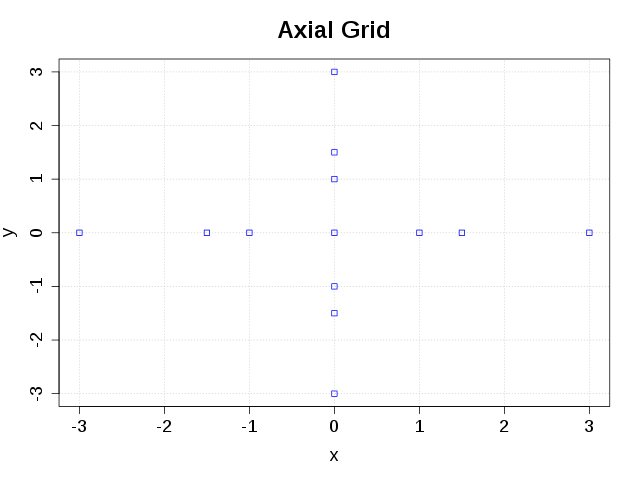
\includegraphics[width=8cm]{Figures/AxialGrid.png}
                   \caption{Axial Design of Experiments  : initial grid.}
                   \label{AxialGrid}
                 \end{center}
               \end{minipage}
               \hfill
               \begin{minipage}{10cm}
                 \begin{center}
                   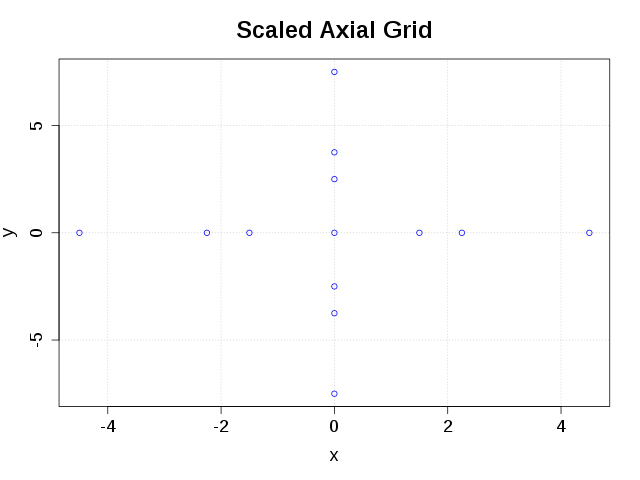
\includegraphics[width=8cm]{Figures/ScaledAxialGrid.png}
                   \caption{Axial Design of Experiments  : after scaling.}
                   \label{ScaledAxialGrid}
                 \end{center}
               \end{minipage}
             \end{figure}

             \begin{figure}[H]
               \begin{center}
                 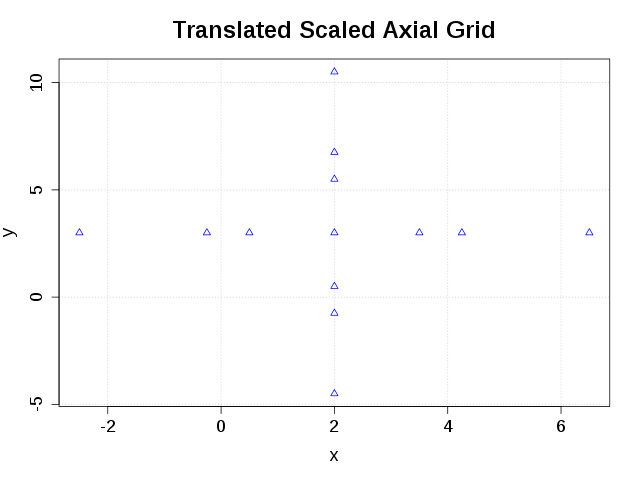
\includegraphics[width=8cm]{Figures/TranslatedScaledAxialGrid.png}
               \end{center}
               \caption{Axial Design of Experiments  : after scaling and translation.}
               \label{TranslatedScaledAxialGrid}
             \end{figure}



             \begin{figure}[H]
               \begin{minipage}{10cm}
                 \begin{center}
                   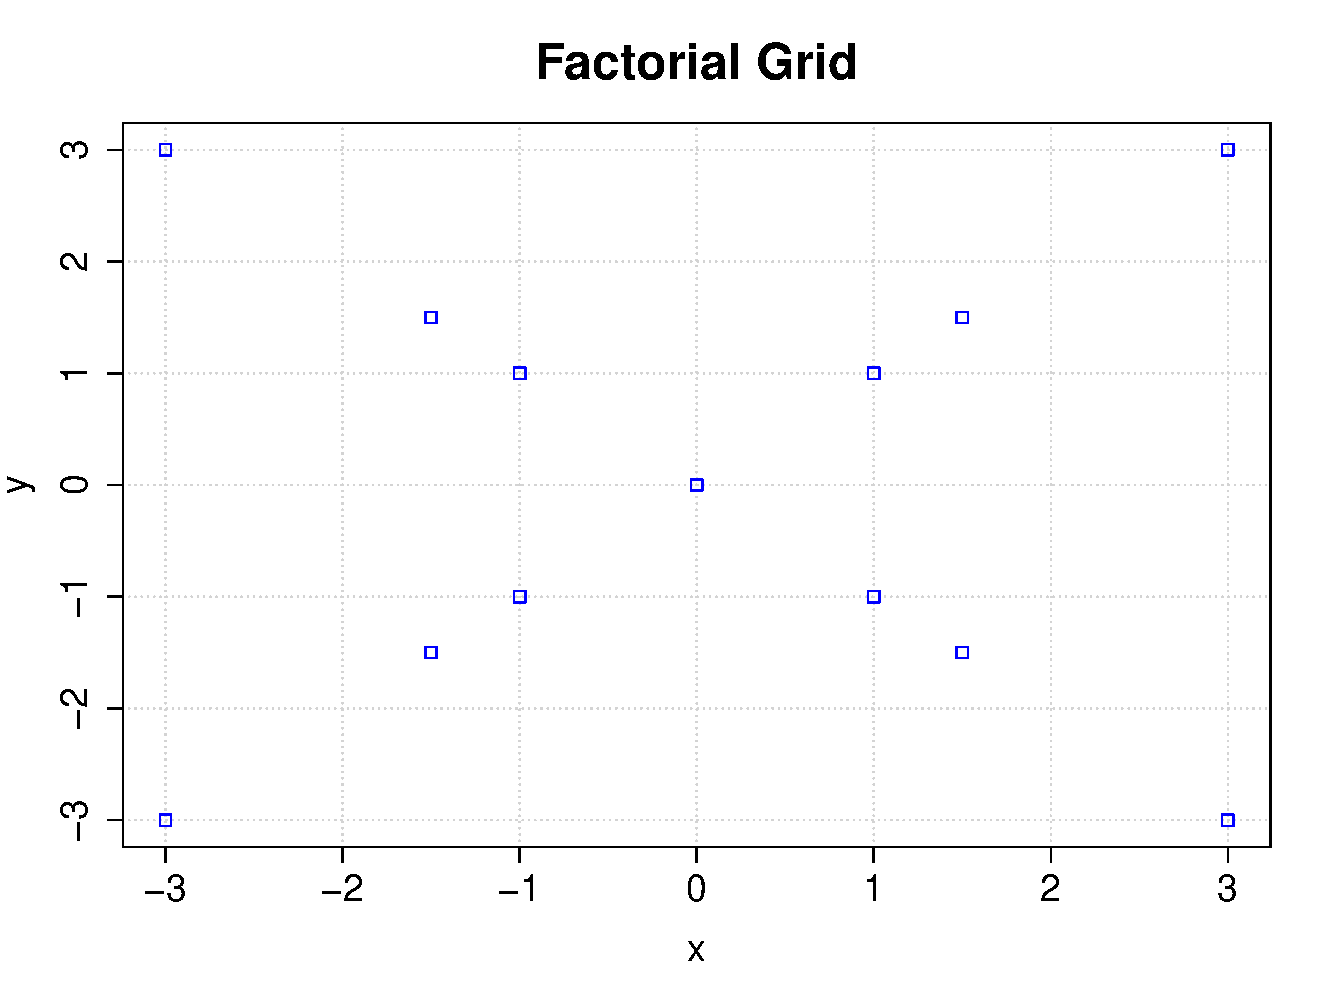
\includegraphics[width=8cm]{Figures/FactorialGrid.pdf}
                   \caption{Factorial Design of Experiments  : initial grid.}
                   \label{FactorialGrid}
                 \end{center}
               \end{minipage}
               \hfill
               \begin{minipage}{10cm}
                 \begin{center}
                   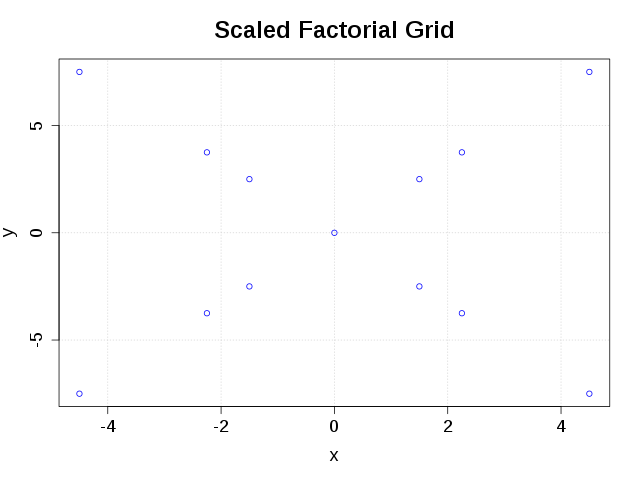
\includegraphics[width=8cm]{Figures/ScaledFactorialGrid.png}
                   \caption{Factorial Design of Experiments  : after scaling.}
                   \label{ScaledFactorialGrid}
                 \end{center}
               \end{minipage}
             \end{figure}




             \begin{figure}[H]
               \begin{center}
                 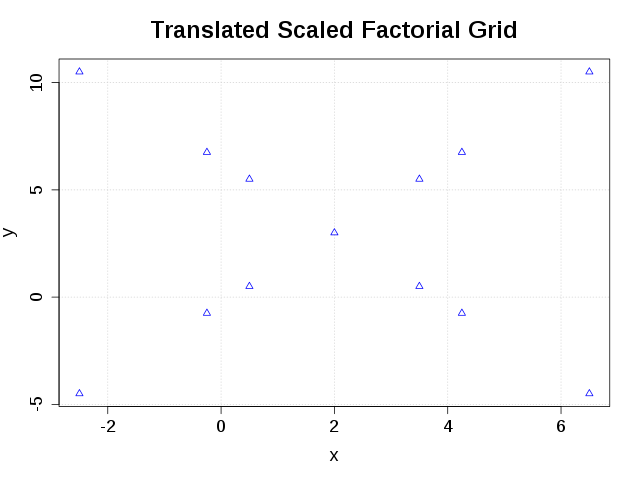
\includegraphics[width=8cm]{Figures/TranslatedScaledFactorialGrid.png}
               \end{center}
               \caption{Factorial Design of Experiments  : after scaling and translation.}
               \label{TranslatedScaledFactorialGrid}
             \end{figure}





             \begin{figure}[H]
               \begin{minipage}{10cm}
                 \begin{center}
                   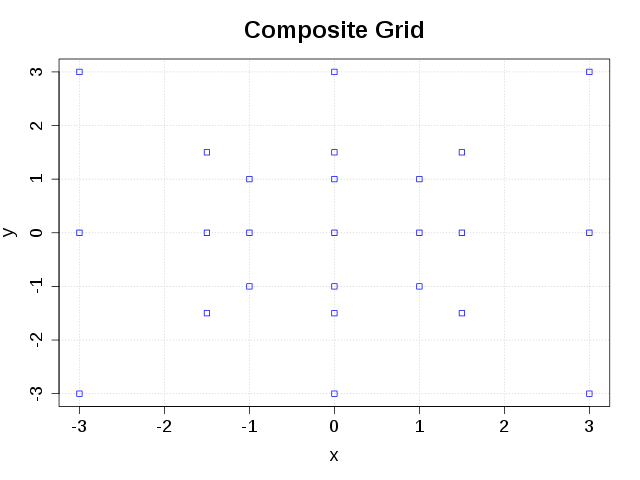
\includegraphics[width=8cm]{Figures/CompositeGrid.png}
                   \caption{Composite Design of Experiments  : initial grid.}
                   \label{CompositeGrid}
                 \end{center}
               \end{minipage}
               \hfill
               \begin{minipage}{10cm}
                 \begin{center}
                   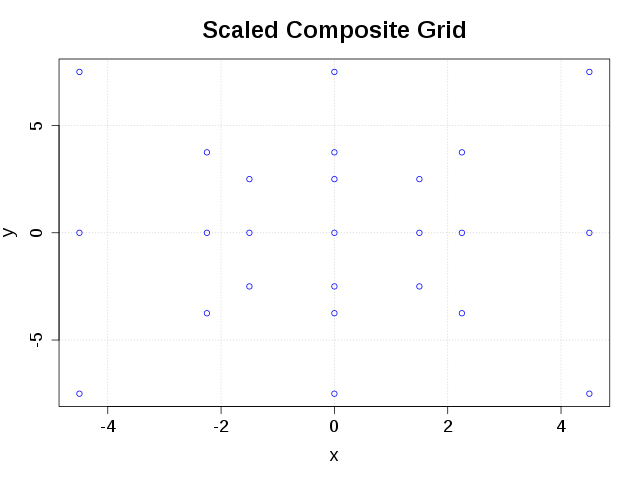
\includegraphics[width=8cm]{Figures/ScaledCompositeGrid.png}
                   \caption{Composite Design of Experiments  : after scaling.}
                   \label{ScaledCompositeGrid}
                 \end{center}
               \end{minipage}
             \end{figure}

             \begin{figure}[H]
               \begin{center}
                 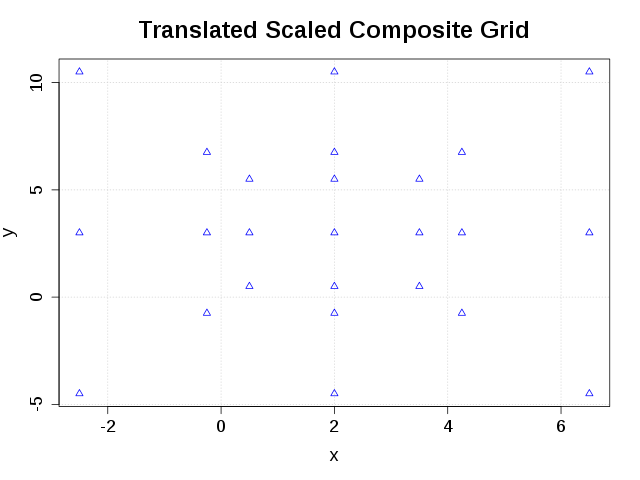
\includegraphics[width=8cm]{Figures/TranslatedScaledCompositeGrid.png}
               \end{center}
               \caption{Composite Design of Experiments  : after scaling and translation.}
               \label{TranslatedScaledCompositeGrid}
             \end{figure}


             \begin{figure}[H]
               \begin{minipage}{10cm}
                 \begin{center}
                   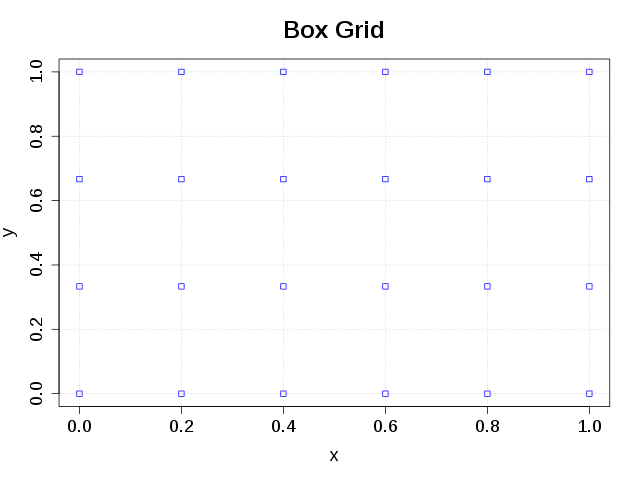
\includegraphics[width=8cm]{Figures/BoxGrid.png}
                   \caption{Box Design of Experiments  : initial grid.}
                   \label{BoxGrid}
                 \end{center}
               \end{minipage}
               \hfill
               \begin{minipage}{10cm}
                 \begin{center}
                   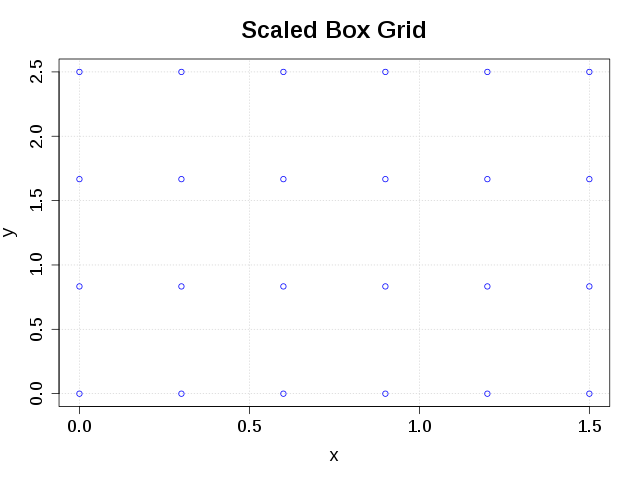
\includegraphics[width=8cm]{Figures/ScaledBoxGrid.png}
                   \caption{Box Design of Experiments  : after scaling.}
                   \label{ScaledBoxGrid}
                 \end{center}
               \end{minipage}
             \end{figure}

             \begin{figure}[H]
               \begin{center}
                 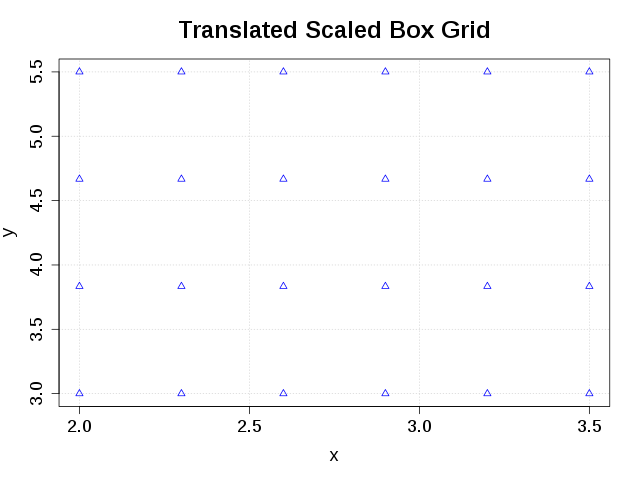
\includegraphics[width=8cm]{Figures/TranslatedScaledBoxGrid.png}
               \end{center}
               \caption{Box Design of Experiments  : after scaling and translation.}
               \label{TranslatedScaledBoxGrid}
             \end{figure}
